%%%%%%%%%%%%%%%%%%%%%% Props %%%%%%%%%%%%%%%%%%%%%%
\documentclass{article}

\usepackage[french]{babel}
\usepackage[utf8]{inputenc}
\usepackage[T1]{fontenc}
\usepackage{graphicx}
\usepackage{fancyhdr}
\usepackage{eurosym}
\usepackage{color}
\usepackage{soul}
\usepackage{listings}
\usepackage{enumitem}
\usepackage{enumerate}
\usepackage{float}

\pagestyle{fancy}
\lhead{Manuel d'utilisation}
\chead{Deadly Science}
\rhead{Custos Carceris}

\title{Manuel d'utilisation}

\begin{document}

\maketitle
\tableofcontents

\newpage
\section{Menus}
\subsection{Menu Principal}

\begin{figure}[H]
	\centering
	
\includegraphics[width=0.49\textwidth]{MainMenu.png}
	\caption{Menu Principal}
	\label{Menu Principal}
\end{figure}

Lorsque vous lancez le jeu vous arriverez sur l'écran principal vous pouvez quitter le jeu, changez les paramètres et entrer dans une salle.
\paragraph{Paramètres}

Sur ce menu, vous pouvez changer vos touches en appuyant sur le bouton de l'action que vous voulez changer de touche, puis appuyez sur la touche de votre choix. Elle devrait s'afficher sur le bouton. Vous pouvez aussi changer de langue en appuyant sur le bouton Langage pui en choissant celle que vous voulez. Vous pouvez aussi changer votre pseudonyme en écrivant le pseudonyme que vous souhaitez ou vous pouvez cliquer sur le bouton Aléatoire pour en créer un de manière aléatoire. A l'aide des barres, vous pouvez changer le volume des sons et musique, et vous pouvez aussi controller la sensibilité de la souris dans le jeu.

\begin{figure}[H]
	\centering
	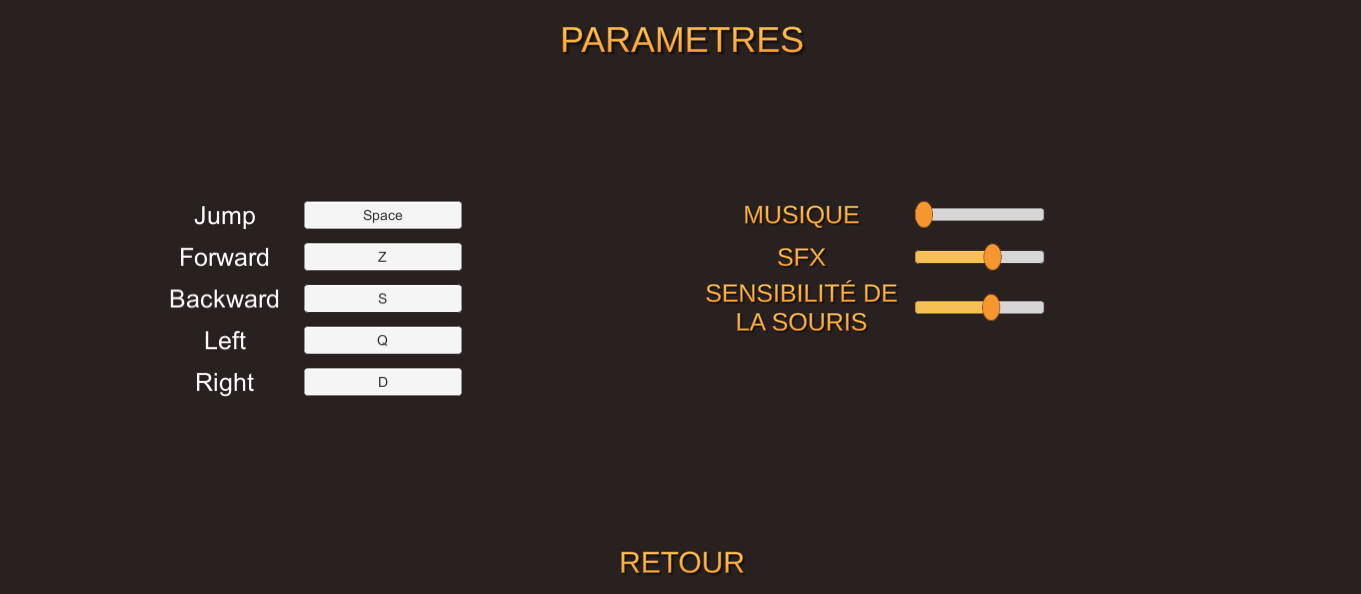
\includegraphics[width=0.49\textwidth]{parametres.png}
	\caption{Paramètres}
	\label{Paramètres}
\end{figure}


\paragraph{}
Lorsque vos paramètres sont configurés vous pouvez cliquer sur Jouer.

\subsection{Enter dans une salle}
Pour entrer dans une salle vous avez deux manières, soit en créer une, soit la rejoindre.
\paragraph{Créer une salle}
Pour créer une salle standard, il suffit de cliquer sur la barre de texte, écrire le nom de la salle que vous souhaitez puis cliquer sur Créer une salle.

\begin{figure}[H]
	\centering
	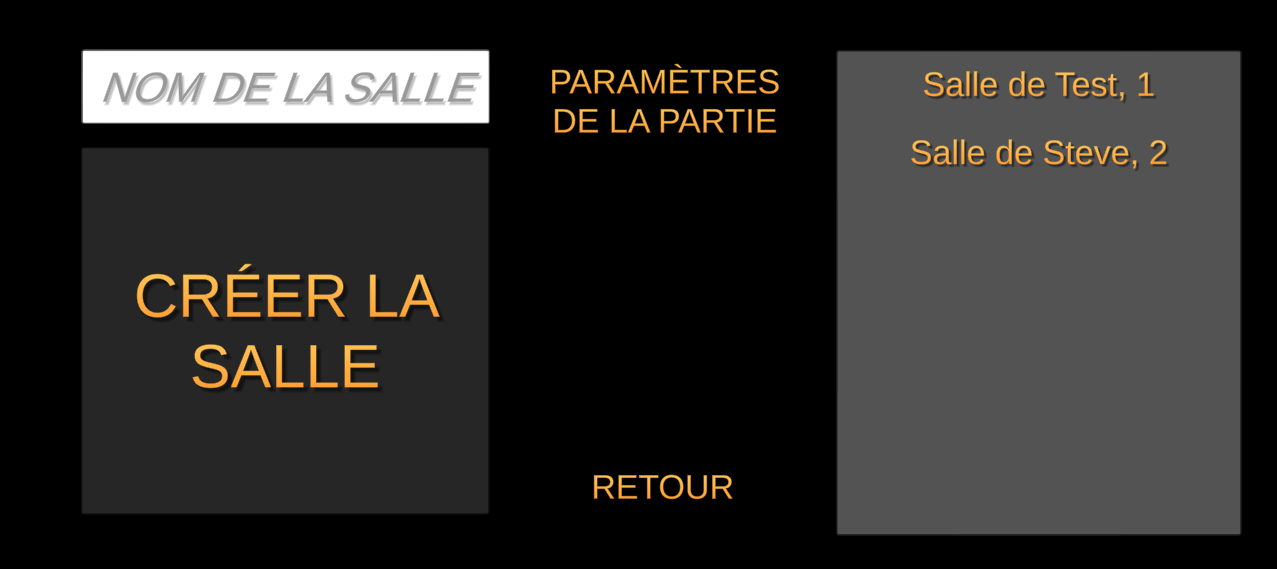
\includegraphics[width=0.49\textwidth]{Menu1.png}
	\caption{Menu pour créer une salle}
	\label{Menu pour créer une salle}
\end{figure}

Si vous voulez une salle avec des paramètres particuliers, vous pouvez cliquer sur Paramètres de la partie, vous serez emmené sur un autre menu.

\begin{figure}[H]
	\centering
	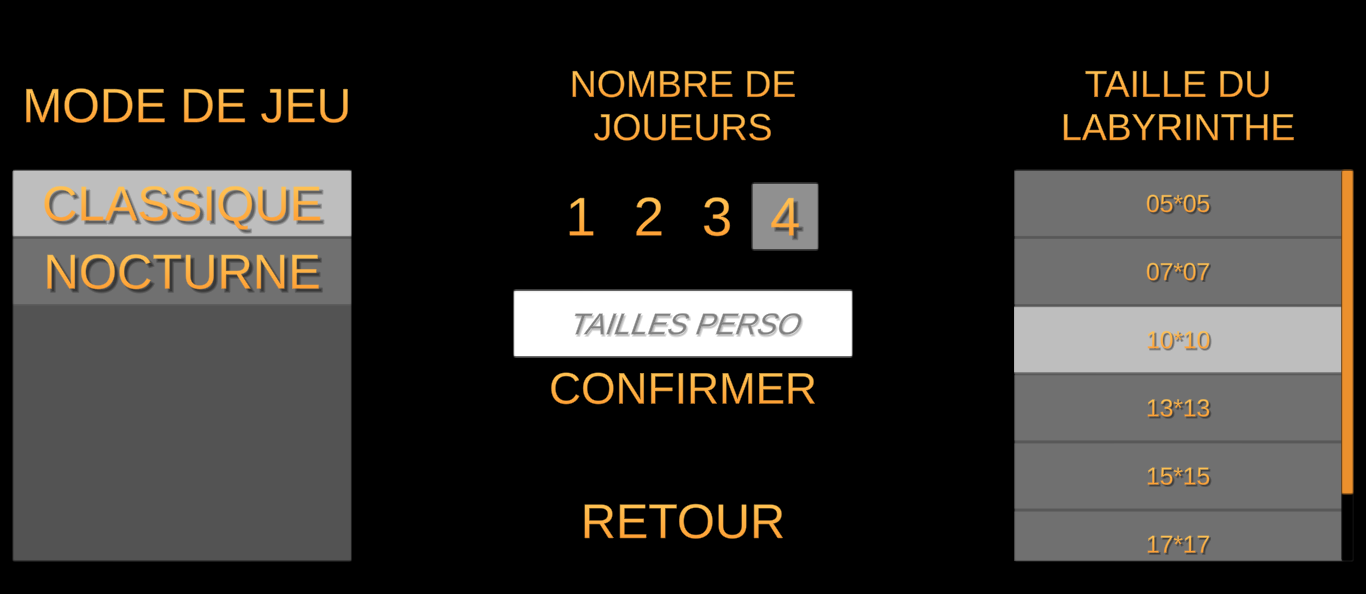
\includegraphics[width=0.49\textwidth]{Menu2.png}
	\caption{Menu pour paramétrer une salle}
	\label{Menu pour paramétrer une salle}
\end{figure}

\paragraph{Configurer une salle}
Sur ce menu vous pouvez changer le nombre de joueurs attendus dans la salle, le mode de jeu de la partie et la taille du labyrinthe. Pour changer le nombre de joueurs dans le labyrinthe, il suffit de cliquer sur le nombre de joueurs que vous souhaitez (le nombre de joueurs influence le jeu). Pour changer le mode de jeu, c'est la même manière, cliquez sur celui que vous souhaitez. Les paramètres choisis ont un fond blanc. 

\paragraph{Changer la taille du labyrinthe}
Pour changer la taille du labyrinthe, vous pouvez soit cliquer sur l'une des tailles du tableau défilant, soit écrire une taille personnalisée dans la barre blanche puis en appuyant sur Confirmer. Assurez vous que vous écrivez la taille du labyrinthe de la bonne manière c'est-à-dire longueur*largeur, sinon vous recevrez un message d'erreur. Si vous voulez choisir une taille prédéfinie qui est en dessous, vous pouvez utiliser la molette pour descendre ou monter sur le tableau défilant. Lorsque vous avez configurer votre salle, vous pouvez appuyer sur Retour et créer une salle.

\paragraph{}
Pour rejoindre une partie, il suffit d'être dans le menu précédant et de cliquer sur la salle que vous souhaitez à droite de l'écran. Vous verez le nom des salles ouvertes ainsi que le nombre de joueurs présents. Si la salle est complète, elle ne sera pas visible. 

\paragraph{A l'intérieur de la salle}
A droite de l'écran, vous pouvez voir la liste des joueurs présents dans la partie. Si vous êtes l'hôte de la salle, vous pouvez commencer la partie que si tous les joueurs présents dans la salle sont prêts (sauf vous évidemment). Vous pouvez voir le statut à côté de leur pseudonyme à droite de l'écran.

\begin{figure}[H]
	\centering
	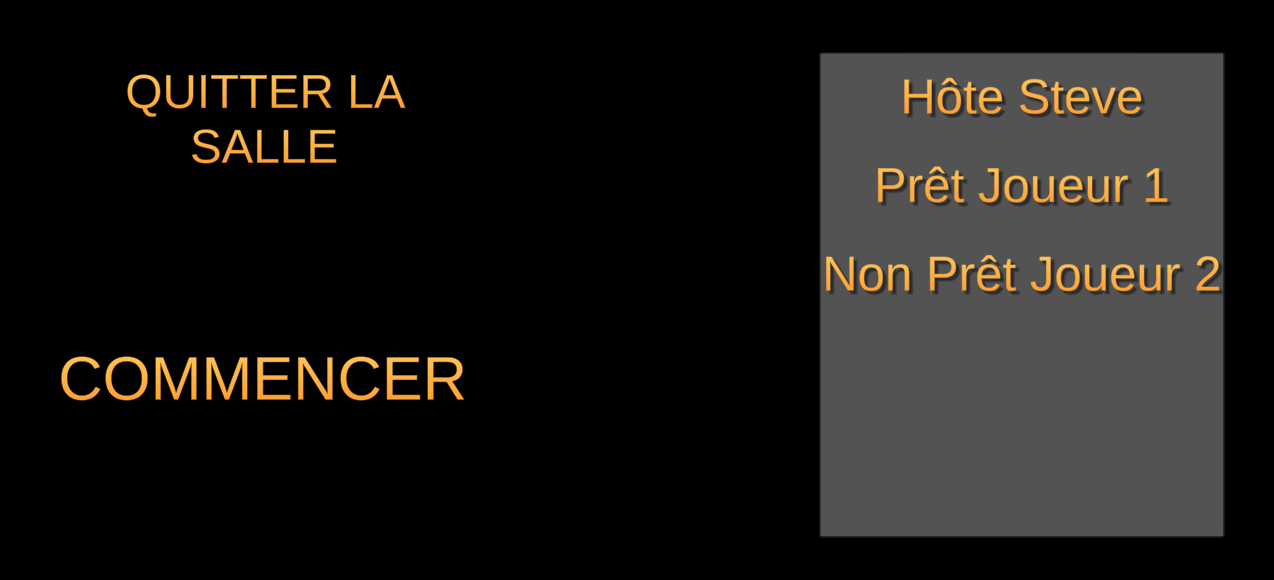
\includegraphics[width=0.49\textwidth]{Menu31.png}
	\caption{Menu lorsque l'on est l'hôte}
	\label{Menu lorsque l'on est l'hôte}
\end{figure}

Si vous ne l'êtes pas, vous pouvez changer changer votre statut en appuyant sur Prêt pour changer votre statut. Le bouton changera en fonction de votre statut. Vous pouvez aussi voir votre statut sur la liste des joueurs à droite de l'écran. 

\begin{figure}[H]
	\centering
	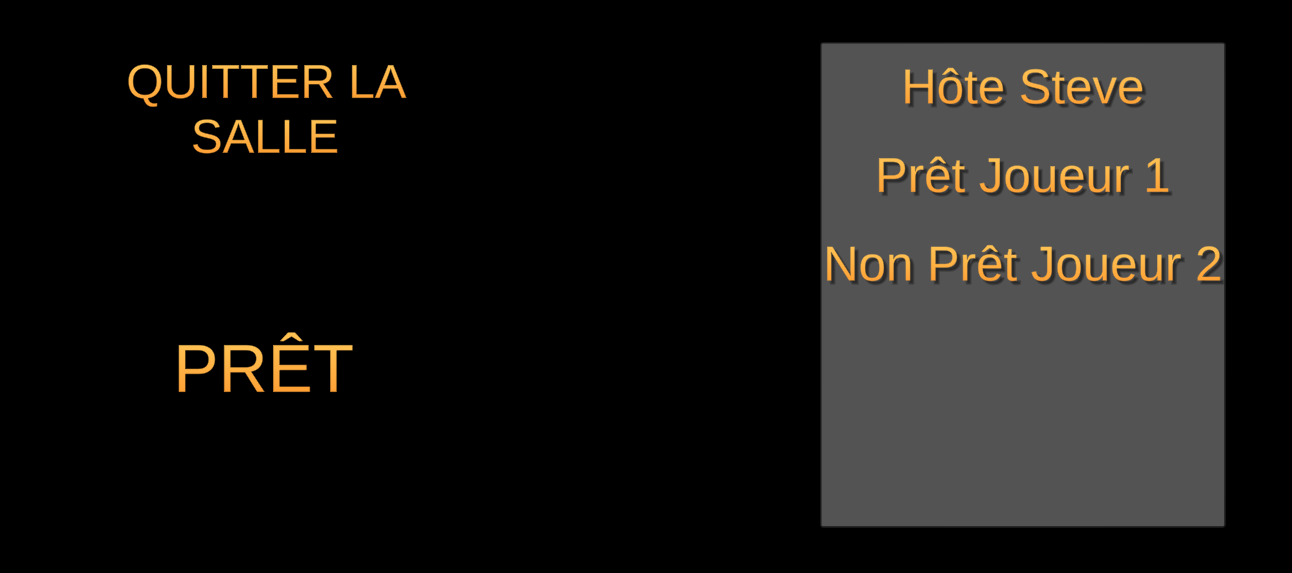
\includegraphics[width=0.49\textwidth]{Menu32.png}
	\caption{Menu lorsque l'on n'est pas l'hôte}
	\label{Menu lorsque l'on n'est pas l'hôte}
\end{figure}

\newpage
\section{Jeu}
\subsection{Première phase}

Lorsque vous êtes en jeu, vous commencez en tant qu'infecté et vous devez chercher un sérum.

\begin{figure}[H]
	\centering
	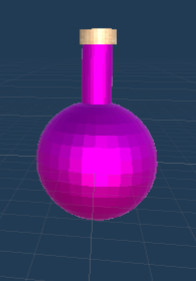
\includegraphics[width=0.49\textwidth]{Fioles.png}
	\caption{Sérum}
	\label{Sérum}
\end{figure}

La mission en cours est affiché en haut à droite de l'écran, votre pseudonyme en haut à gauche de l'écran, les objets qui sont actifs sur vous en bas à droite de l'écran. Vous pouvez savoir votre statut en fonction de la couleur de votre pesudonyme : violet infecté, gris fantôme, vert guéri, rouge corrompu. 

\begin{figure}[H]
	\centering
	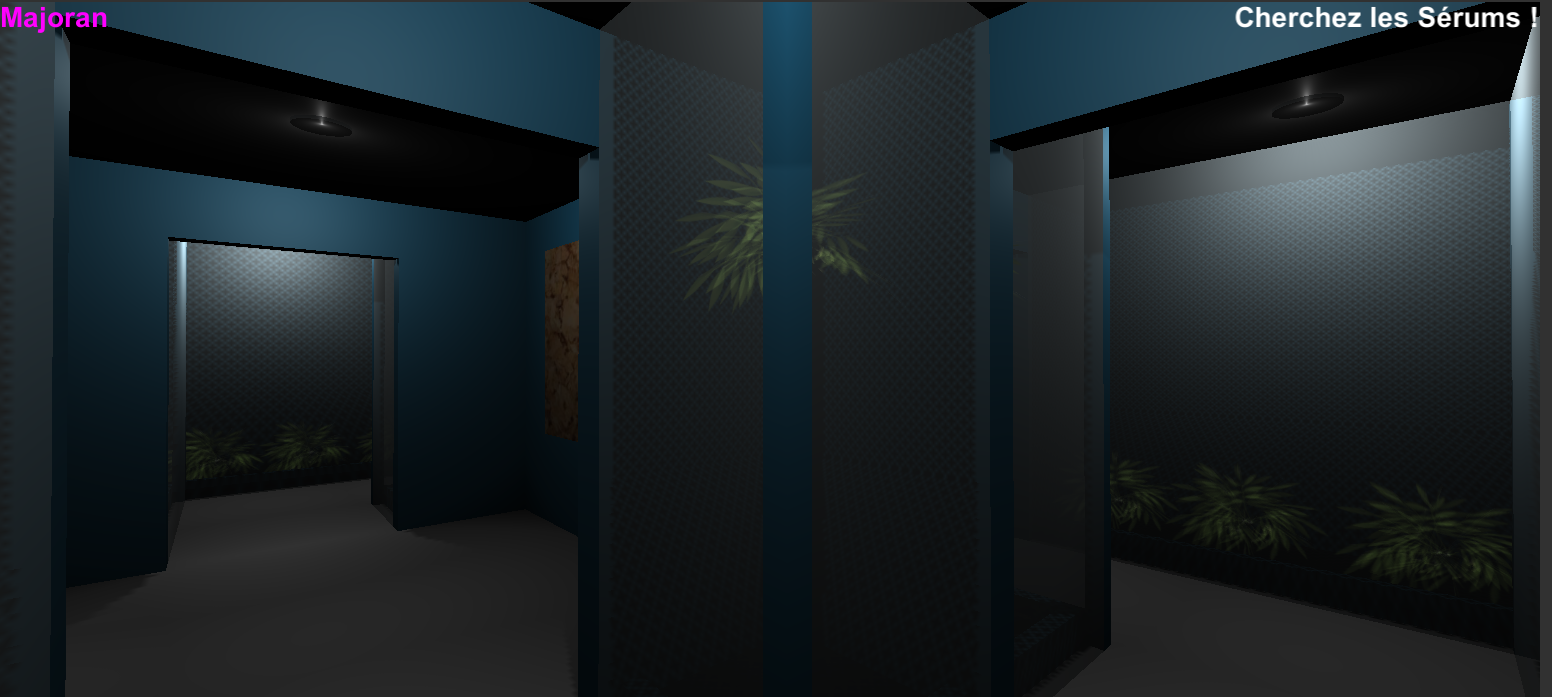
\includegraphics[width=0.49\textwidth]{Lumieres.png}
	\caption{A l'intérieur de la partie}
	\label{A l'intérieur de la partie}
\end{figure}

A l'aide des touches configurés dans les paramètres, vous pouvez vous déplacer dans le labyrinthe. Si vous voulez les changer en pleine partie, il vous suffit d'appuyer sur le bouton Echap et de les configurer de nouveau. A noter que vu que le jeu est synchronisé en réseau, les autres joueurs continuent à jouer pendant que vous êtes dans ce menu. Lorsqu'un joueur est à proximité et en face de vous, vous pouvez lui envoyer un coup de poing en faisant un clic gauche. Ceci lui fera baissez sa barre d'endurance. Lorsque sa barre est à zero, il sera ralenti et ne pourra plus se battre pendant un certain temps.

\subsection{Deuxième phase}

Lorsque tous les joueurs sauf un (à part si vous jouez seul) sont guéris, les joueurs guéris doivent échapper au corrompu et le corrompu doit les contaminer. Pour cela, le corrompu peut soit les toucher, soit les frapper. Lorsque le minuteur affiché en haut à gauche du GUI arrive à zero et que tous les joueurs ne sont pas corrompus, les joueurs guéris gagnent. En revanche si tous les joueurs guéris sont corrompu avant la fin du décompte, le joueur corrompu gagne et les autres perdent. Lorsqu'un joueur devient corrompu, il doit aider les autres joueurs corrompu à contaminer les joueurs guéris.

Pour aider les joueurs, il existe multiples objets qui sont affichés comme montré sur la Figure 9 pour vous aider ou vous ralentir dans votre quête. La liste des objets ainsi que leurs effets sont inscris sur notre site Web dans la partie Codex Plaga. 

\begin{figure}[H]
	\centering
	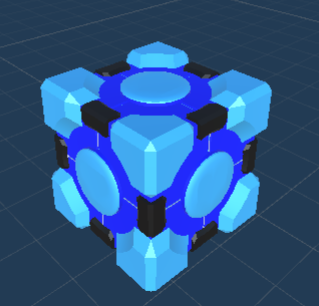
\includegraphics[width=0.49\textwidth]{Objet.png}
	\caption{Objet}
	\label{Objet}
\end{figure}

Lorsque vous arrivez à l'écran de victoire ou de défaite, vous pouvez cliquer sur Quitter pour quitter le jeu. Pour recommencer, il suffit de relancer le jeu.

Bonne chance dans Deadly Science !
\end{document}
